\documentclass[tikz,border=12pt]{standalone}
\usepackage[T1]{fontenc}
\usepackage{mathpazo}
\usepackage{amsmath,amssymb}
\usetikzlibrary{arrows.meta, positioning, calc}

\definecolor{stblue}{HTML}{7B97AD}
\definecolor{rwgold}{HTML}{B8995E}
\definecolor{sage}{HTML}{7A9A7E}
\definecolor{dkbrown}{HTML}{3D3530}
\definecolor{wmgray}{HTML}{7B7067}
\definecolor{cream}{HTML}{F9F6F0}
\definecolor{border}{HTML}{D4C9B8}
\definecolor{terracotta}{HTML}{C47A6A}
\definecolor{lavender}{HTML}{907EA0}

\begin{document}
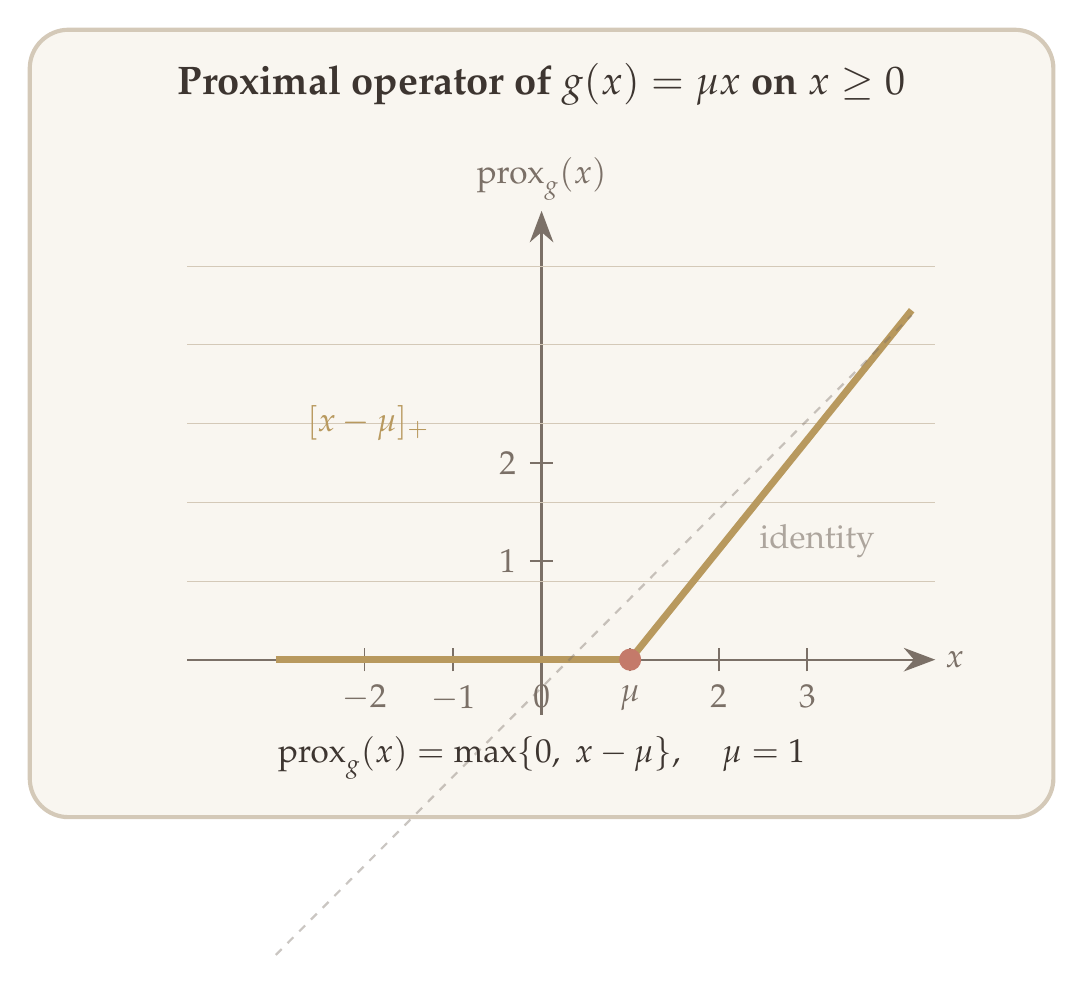
\begin{tikzpicture}[>={Stealth[length=4mm, width=3mm]}]

% Background
\fill[cream, rounded corners=14pt] (-0.5,-0.5) rectangle (12.5,9.5);
\draw[border, line width=1.5pt, rounded corners=14pt] (-0.5,-0.5) rectangle (12.5,9.5);

% Title
\node[text=dkbrown, font=\Large\bfseries] at (6,8.8)
  {Proximal operator of $g(x) = \mu x$ on $x \geq 0$};

% Axes
\draw[wmgray, line width=0.8pt, ->] (1.5,1.5) -- (11,1.5) node[right, font=\large, text=wmgray] {$x$};
\draw[wmgray, line width=0.8pt, ->] (6,0.8) -- (6,7.2) node[above, font=\large, text=wmgray] {$\operatorname{prox}_g(x)$};

% Grid lines (light)
\foreach \y in {2.5,3.5,4.5,5.5,6.5} {
  \draw[border, line width=0.3pt] (1.5,\y) -- (11,\y);
}

% Tick marks on x-axis: range -3 to 5, centered at x=6, scale 1 unit = 1.125cm
% mu = 1, so breakpoint at x=1 -> position 6 + 1*1.125 = 7.125
% x-axis: x_val -> 6 + x_val * 1.125
% y-axis: y_val -> 1.5 + y_val * 1.25

% Tick marks
\draw[wmgray, line width=0.6pt] (6,1.35) -- (6,1.65);
\node[text=wmgray, font=\large, below] at (6,1.3) {$0$};

% mu = 1 mark
\draw[wmgray, line width=0.6pt] (7.125,1.35) -- (7.125,1.65);
\node[text=wmgray, font=\large, below] at (7.125,1.3) {$\mu$};

% Negative ticks
\draw[wmgray, line width=0.6pt] (4.875,1.35) -- (4.875,1.65);
\node[text=wmgray, font=\large, below] at (4.875,1.3) {$-1$};
\draw[wmgray, line width=0.6pt] (3.75,1.35) -- (3.75,1.65);
\node[text=wmgray, font=\large, below] at (3.75,1.3) {$-2$};

% Positive ticks
\draw[wmgray, line width=0.6pt] (8.25,1.35) -- (8.25,1.65);
\node[text=wmgray, font=\large, below] at (8.25,1.3) {$2$};
\draw[wmgray, line width=0.6pt] (9.375,1.35) -- (9.375,1.65);
\node[text=wmgray, font=\large, below] at (9.375,1.3) {$3$};

% Y-axis ticks
\draw[wmgray, line width=0.6pt] (5.85,2.75) -- (6.15,2.75);
\node[text=wmgray, font=\large, left] at (5.8,2.75) {$1$};
\draw[wmgray, line width=0.6pt] (5.85,4.0) -- (6.15,4.0);
\node[text=wmgray, font=\large, left] at (5.8,4.0) {$2$};

% Function: prox_g(x) = max(0, x - mu) with mu=1
% For x <= 1: y = 0  (horizontal line at y=0, i.e., at canvas y=1.5)
% For x >= 1: y = x - 1 (line with slope 1)

% Flat part: from x=-3 to x=1 -> canvas (2.625, 1.5) to (7.125, 1.5)
\draw[rwgold, line width=2.5pt] (2.625,1.5) -- (7.125,1.5);

% Rising part: from x=1 to x=4.5 -> y=0 to y=3.5
% canvas: (7.125, 1.5) to (6 + 4.5*1.125, 1.5 + 3.5*1.25) = (11.0625, 5.875)
\draw[rwgold, line width=2.5pt] (7.125,1.5) -- (10.7,5.9375);

% Breakpoint marker
\fill[terracotta] (7.125,1.5) circle (4pt);

% Identity line (dashed, for reference)
\draw[wmgray, line width=0.8pt, dashed, opacity=0.4]
  (2.625, {1.5 + (-3)*1.25}) -- (10.7, {1.5 + 3.5*1.25});

% Legend / annotation
\node[text=rwgold, font=\large] at (3.8,4.5) {$[x - \mu]_+$};
\node[text=wmgray, font=\large, opacity=0.6] at (9.5,3.0) {identity};

% Formula
\node[text=dkbrown, font=\large] at (6,0.25)
  {$\operatorname{prox}_g(x) = \max\{0,\; x - \mu\}$, \quad $\mu = 1$};

\end{tikzpicture}
\end{document}
